\section{Hazard of Overfitting}
\noindent
{\color{LightRubineRed} \rule{\linewidth}{1mm} }
\subsection{What is Overfitting} % (fold)
\label{sub:what_is_overfitting}
\textcolor{mypink2}{Hazard} : 冒险 \par
\textbf{Bad Generalizaton} \par
low $E_{in}$,high $E_{out}$. \par
\begin{myremark}{}
不管模型多复杂$M$,或者数据量多少$N$,其实就以下两个考虑。 \par
\begin{align*}
\mathbb{E}_{out} \approx \mathbb{E}_{in} \approx 0 \\
\end{align*}
即使$E+{in}$非常小有什么用?作为预测使用我们需要的是$E_{out}$。
\end{myremark}
下图揭示了模型大小,与数据量大小的关系。 \par
\begin{center}
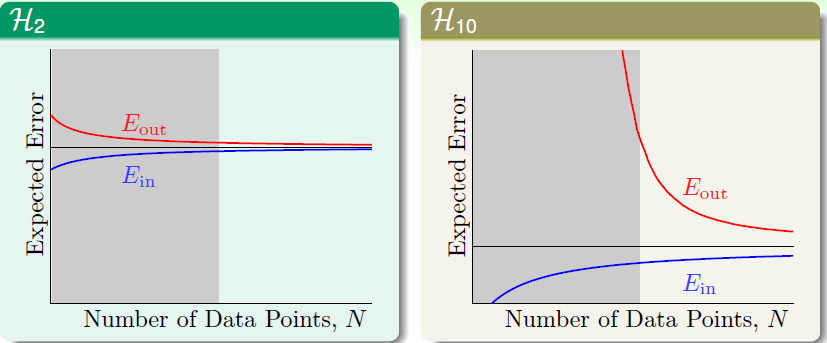
\includegraphics[width=10cm, height=5cm]{lecture13_1}\\
\end{center}
% subsection what_is_overfitting (end)

\subsection{Dealing with Overfitting} % (fold)
\label{sub:dealing_with_overfitting}
\begin{center}
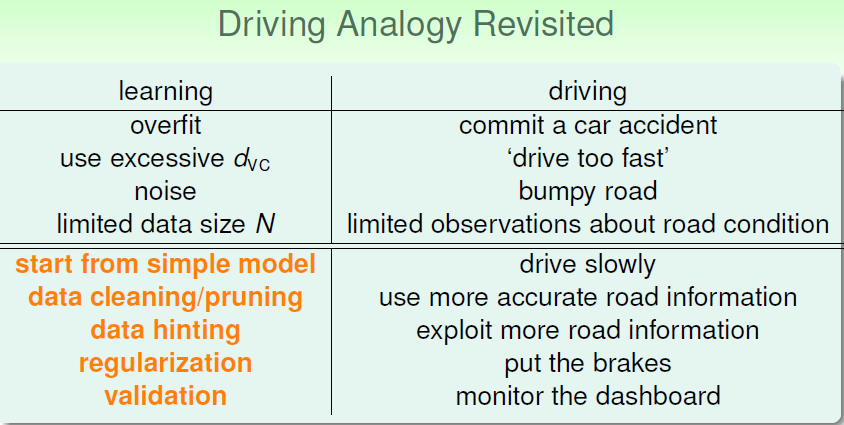
\includegraphics[width=10cm, height=6cm]{lecture13_2}\\
\end{center}
% subsection dealing_with_overfitting (end)
\begin{center}
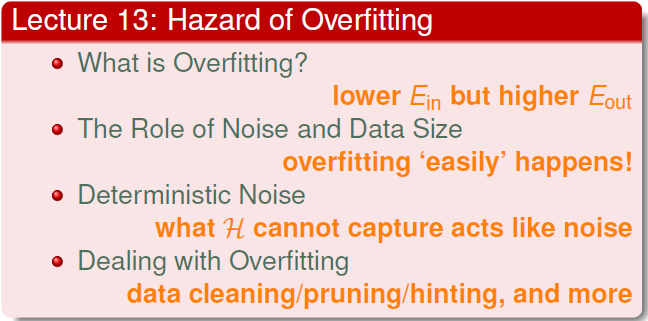
\includegraphics[width=10cm, height=5cm]{lecture13_sum}\\
\end{center}
\noindent
{\color{RubineRed} \rule{\linewidth}{1mm} }